%%%%%%%%%%%%%%%%%%%%%%%%%%%%%%%%%%%%%%%%%%%%%%%%%%%%%%%%%%%%%%%%%%%%%
%% This is a (brief) model paper using the achemso class
%% The document class accepts keyval options, which should include
%% the target journal and optionally the manuscript type. 
%%%%%%%%%%%%%%%%%%%%%%%%%%%%%%%%%%%%%%%%%%%%%%%%%%%%%%%%%%%%%%%%%%%%%
\documentclass[journal=jacsat,manuscript=article]{achemso}
\usepackage{subcaption}
\usepackage{amsmath}
\usepackage{graphicx}
\usepackage{array}
\usepackage{adjustbox}
\usepackage{longtable}
\usepackage{xcolor}
\usepackage[normalem]{ulem} 
%\usepackage[version=3]{mhchem} % Formula subscripts using \ce{}

%%%%%%%%%%%%%%%%%%%%%%%%%%%%%%%%%%%%%%%%%%%%%%%%%%%%%%%%%%%%%%%%%%%%%
%% If issues arise when submitting your manuscript, you may want to
%% un-comment the next line.  This provides information on the
%% version of every file you have used.
%%%%%%%%%%%%%%%%%%%%%%%%%%%%%%%%%%%%%%%%%%%%%%%%%%%%%%%%%%%%%%%%%%%%%
%%\listfiles

%%%%%%%%%%%%%%%%%%%%%%%%%%%%%%%%%%%%%%%%%%%%%%%%%%%%%%%%%%%%%%%%%%%%%
%% Place any additional macros here.  Please use \newcommand* where
%% possible, and avoid layout-changing macros (which are not used
%% when typesetting).
%%%%%%%%%%%%%%%%%%%%%%%%%%%%%%%%%%%%%%%%%%%%%%%%%%%%%%%%%%%%%%%%%%%%%
\newcommand*\mycommand[1]{\texttt{\emph{#1}}}

%%%%%%%%%%%%%%%%%%%%%%%%%%%%%%%%%%%%%%%%%%%%%%%%%%%%%%%%%%%%%%%%%%%%%
%% Meta-data block
%% ---------------
%% Each author should be given as a separate \author command.
%%
%% Corresponding authors should have an e-mail given after the author
%% name as an \email command. Phone and fax numbers can be given
%% using \phone and \fax, respectively; this information is optional.
%%
%% The affiliation of authors is given after the authors; each
%% \affiliation command applies to all preceding authors not already
%% assigned an affiliation.
%%
%% The affiliation takes an option argument for the short name.  This
%% will typically be something like "University of Somewhere".
%%
%% The \altaffiliation macro should be used for new address, etc.
%% On the other hand, \alsoaffiliation is used on a per author basis
%% when authors are associated with multiple institutions.
%%%%%%%%%%%%%%%%%%%%%%%%%%%%%%%%%%%%%%%%%%%%%%%%%%%%%%%%%%%%%%%%%%%%%
\author{Juan Gomez Quispe}
\affiliation[Universidade Federal do ABC]
{Center of Natural and Human Sciences, Federal University of ABC, Santo André, São Paulo, Brazil}

\author{Caique Campos de Oliveira}
\affiliation[Universidade Federal do ABC]
{Center of Natural and Human Sciences, Federal University of ABC, Santo André, São Paulo, Brazil}

\author{Carlos Raul Primo Sapillado}
\affiliation[National University of San Marcos]
{Facultad de Ciencias Físicas, Universidad Nacional Mayor de San Marcos, 15081 Lima, Perú}

\author{C Rojas-Ayala}
\affiliation[National University of San Marcos]
{Facultad de Ciencias Físicas, Universidad Nacional Mayor de San Marcos, 15081 Lima, Perú}

\author{Pedro Alves Da Silva Autreto}
\affiliation[Universidade Federal do ABC]
{Center of Natural and Human Sciences, Federal University of ABC, Santo André, São Paulo, Brazil}

\email{pedro.autreto@ufabc.edu.br}
\phone{+55 (19) 98279-4988}

%%%%%%%%%%%%%%%%%%%%%%%%%%%%%%%%%%%%%%%%%%%%%%%%%%%%%%%%%%%%%%%%%%%%%
%% The document title should be given as usual. Some journals require
%% a running title from the author: this should be supplied as an
%% optional argument to \title.
%%%%%%%%%%%%%%%%%%%%%%%%%%%%%%%%%%%%%%%%%%%%%%%%%%%%%%%%%%%%%%%%%%%%%
\title[An \textsf{achemso} demo]
  {
Coordination-Dependent Hydrogen Adsorption on Co-, Fe-, and Ni-Functionalized Monolayer CrCl$_{3}$
  }

%%%%%%%%%%%%%%%%%%%%%%%%%%%%%%%%%%%%%%%%%%%%%%%%%%%%%%%%%%%%%%%%%%%%%
%% Some journals require a list of abbreviations or keywords to be
%% supplied. These should be set up here, and will be printed after
%% the title and author information, if needed.
%%%%%%%%%%%%%%%%%%%%%%%%%%%%%%%%%%%%%%%%%%%%%%%%%%%%%%%%%%%%%%%%%%%%%
\setkeys{acs}{keywords = true} 
\abbreviations{2d-CrCl$_{3}$, TMF, HA, magnetic-2d}
\keywords{Monolayer-CrCl$_{3}$, Transition-metal functionalization, Hydrogen Adsorption, Magnetic two-dimensional materials}

%%%%%%%%%%%%%%%%%%%%%%%%%%%%%%%%%%%%%%%%%%%%%%%%%%%%%%%%%%%%%%%%%%%%%
%% The manuscript does not need to include \maketitle, which is
%% executed automatically.
%%%%%%%%%%%%%%%%%%%%%%%%%%%%%%%%%%%%%%%%%%%%%%%%%%%%%%%%%%%%%%%%%%%%%
\begin{document}

\begin{suppinfo}

\begin{figure}[H]
    \centering
    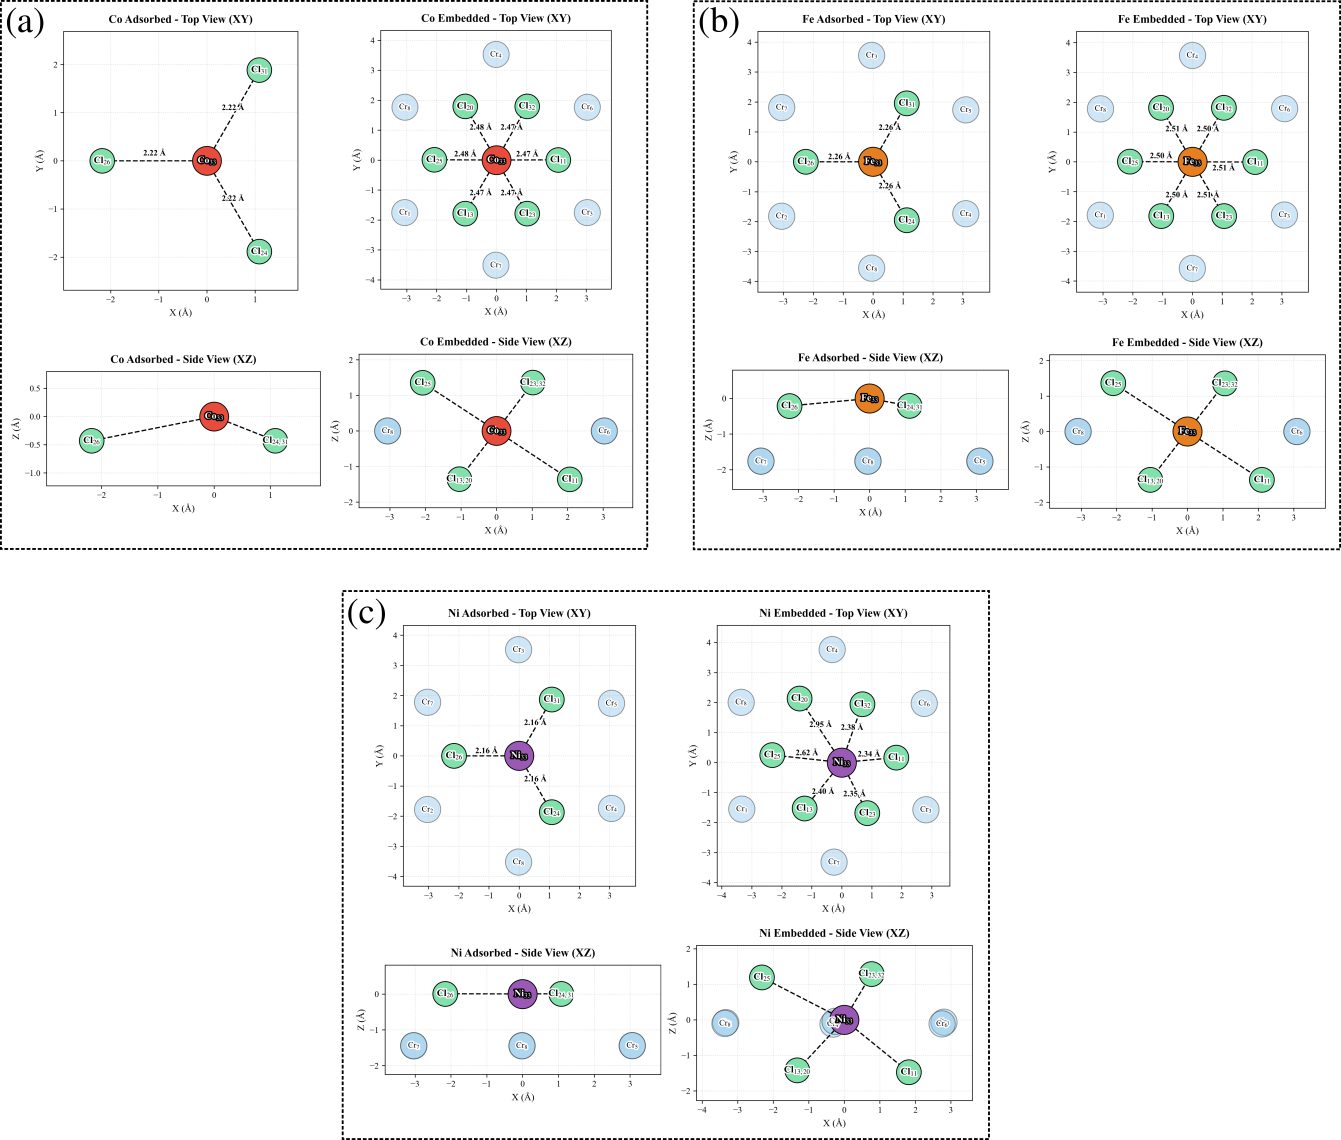
\includegraphics[width=1.0\linewidth]{figure/new_sup_fig_1.png}
        \caption*{Fig. S1. Schematic top ($XY$) and side ($XZ$) views of the optimized local coordination geometries and TM--Cl bond lengths (\AA) for (a) Co-, (b) Fe-, and (c) Ni-functionalized monolayer CrCl$_3$ in both adsorbed (hollow site, 3-fold coordinated) and embedded (6-fold octahedrally coordinated) configurations. Light blue, light green, and red/orange/purple spheres represent Cr, Cl, and transition-metal (Co, Fe, Ni) atoms, respectively.}
        \label{fig:S1}
\end{figure}

\begin{figure}[H]
    \centering
    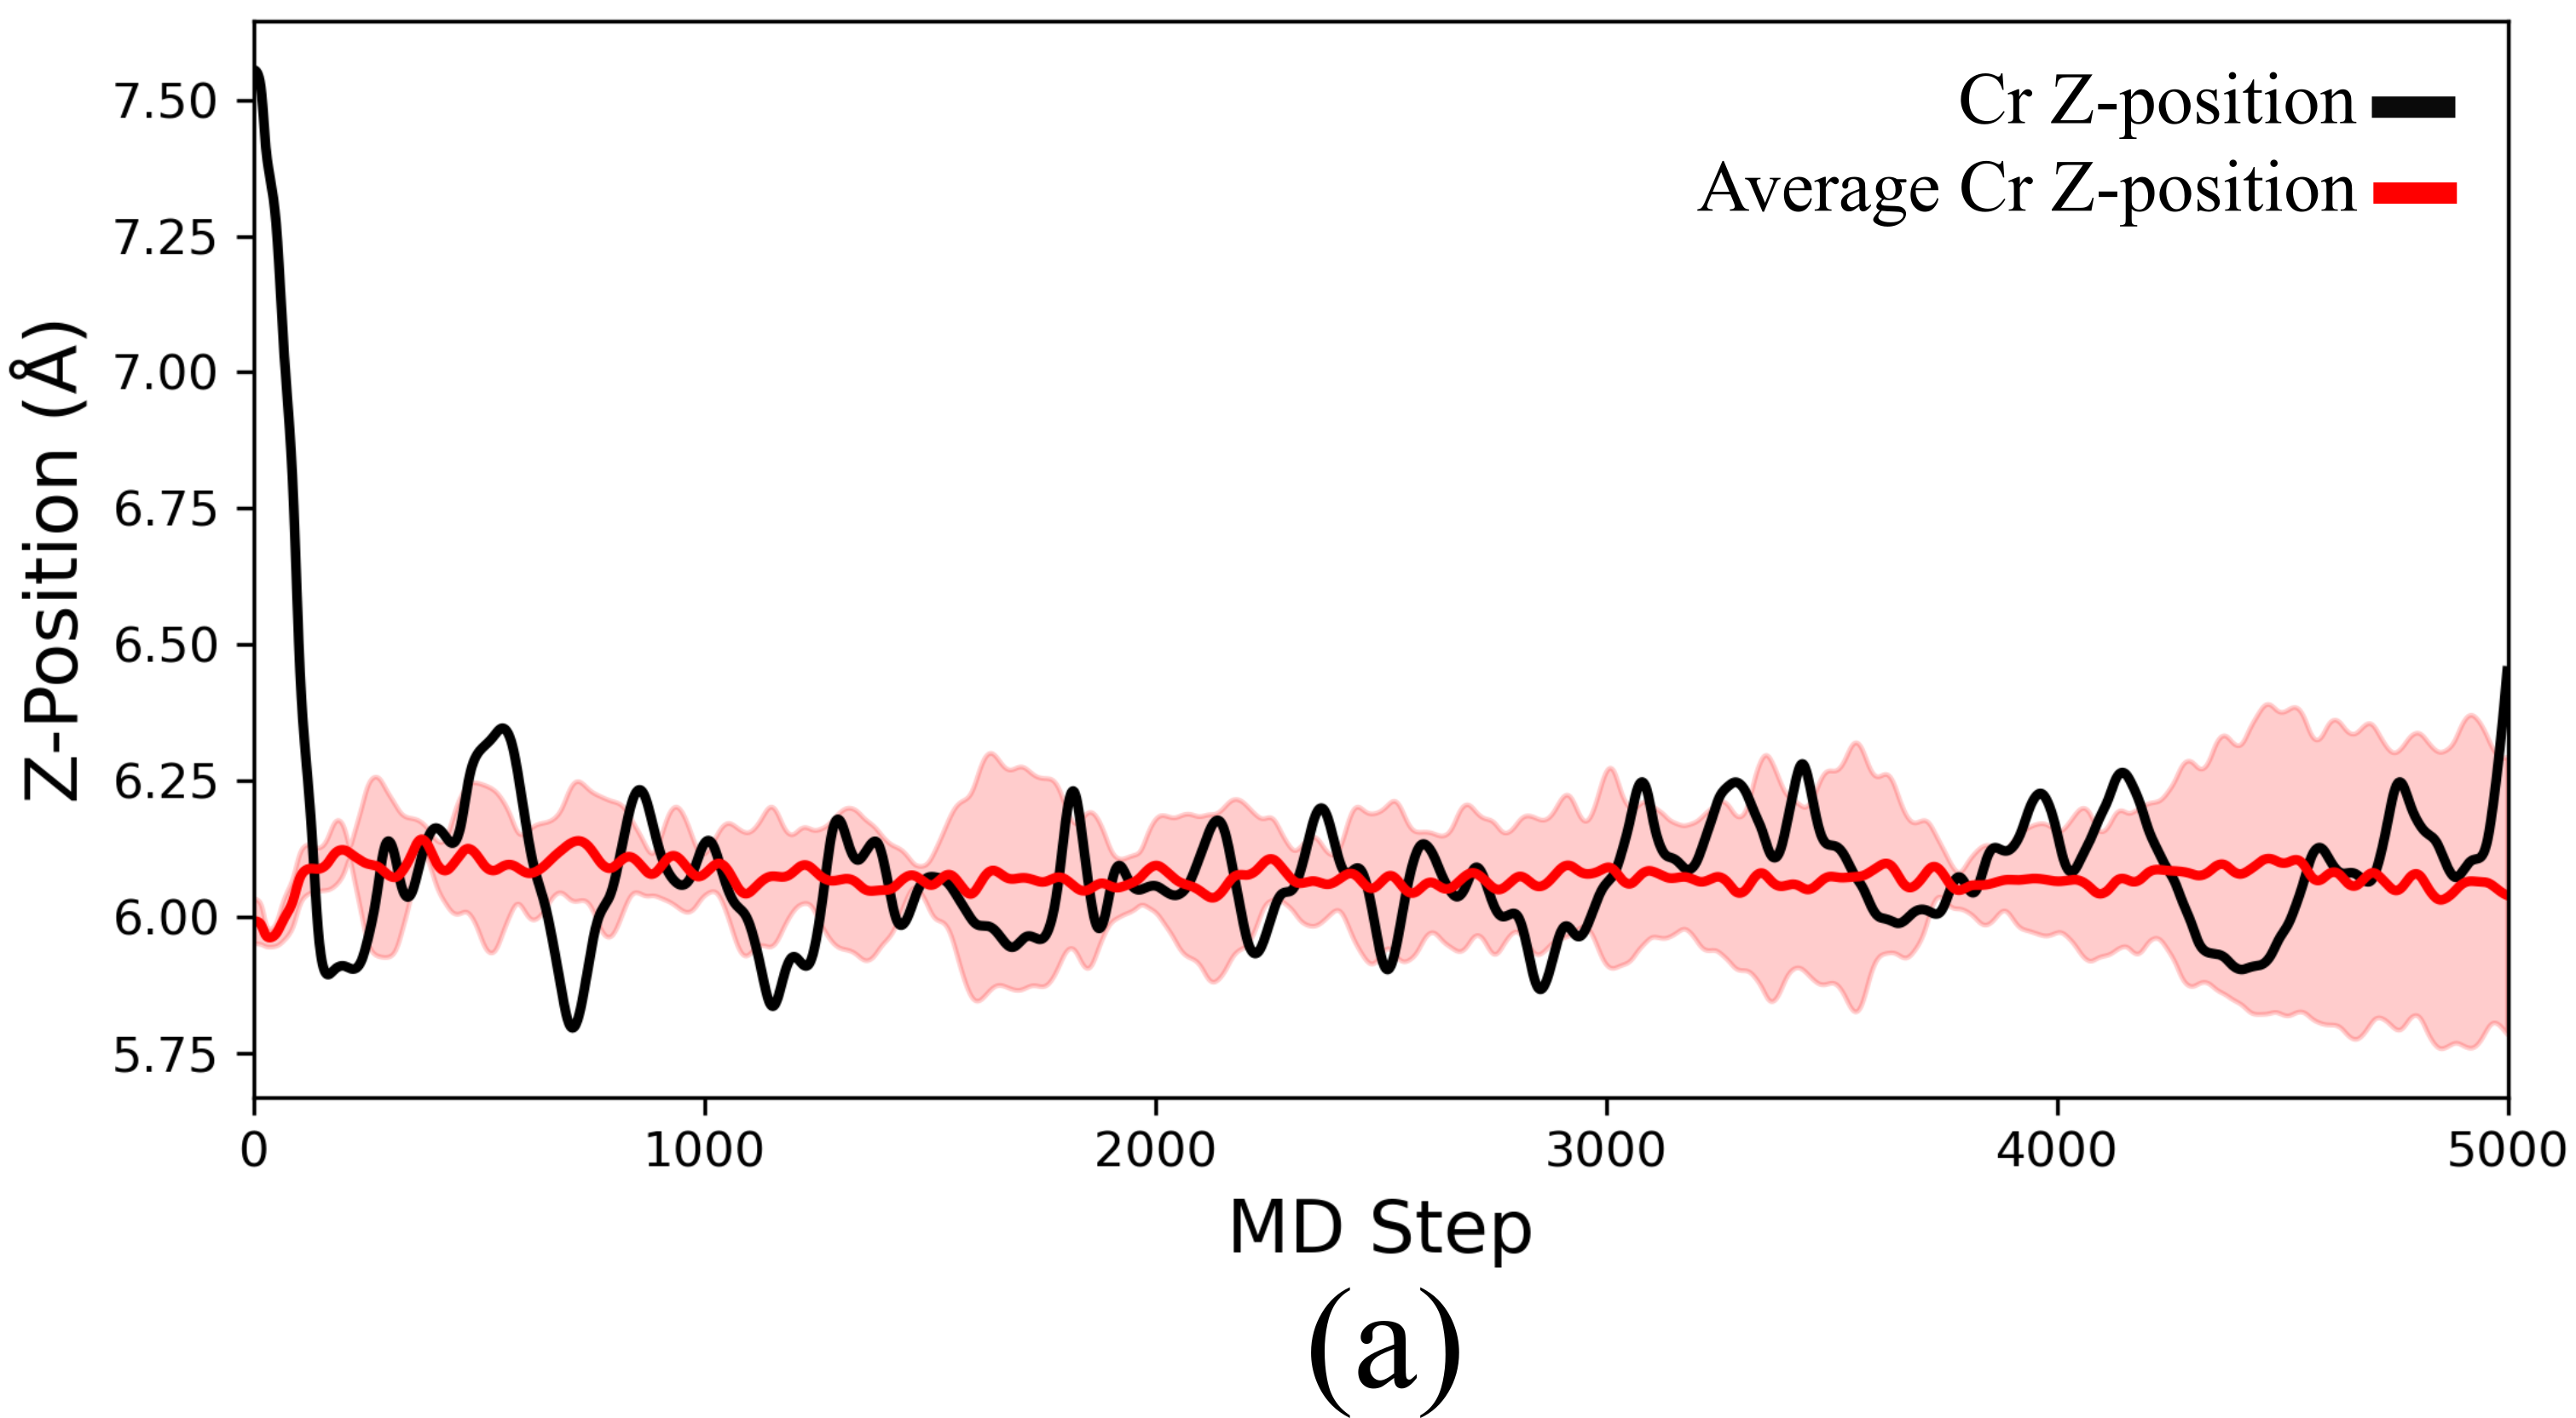
\includegraphics[width=1.0\linewidth]{figure/Fig_SI_2.png}
    \caption*{Fig. S2. Time evolution of the absolute $z$ coordinate of the Cr atom initially adsorbed at the hollow site of monolayer CrCl$_3$ during a 5~ps \textit{ab initio}
    molecular dynamics simulation at 300~K. The black curve
    represents the instantaneous $z$ coordinate of the
    adsorbed Cr atom, whereas the red curve denotes the average
    $z$ coordinate of the Cr atoms belonging to the host
    monolayer.}
    \label{fig:S2}
\end{figure}

\begin{figure}[H]
    \centering
    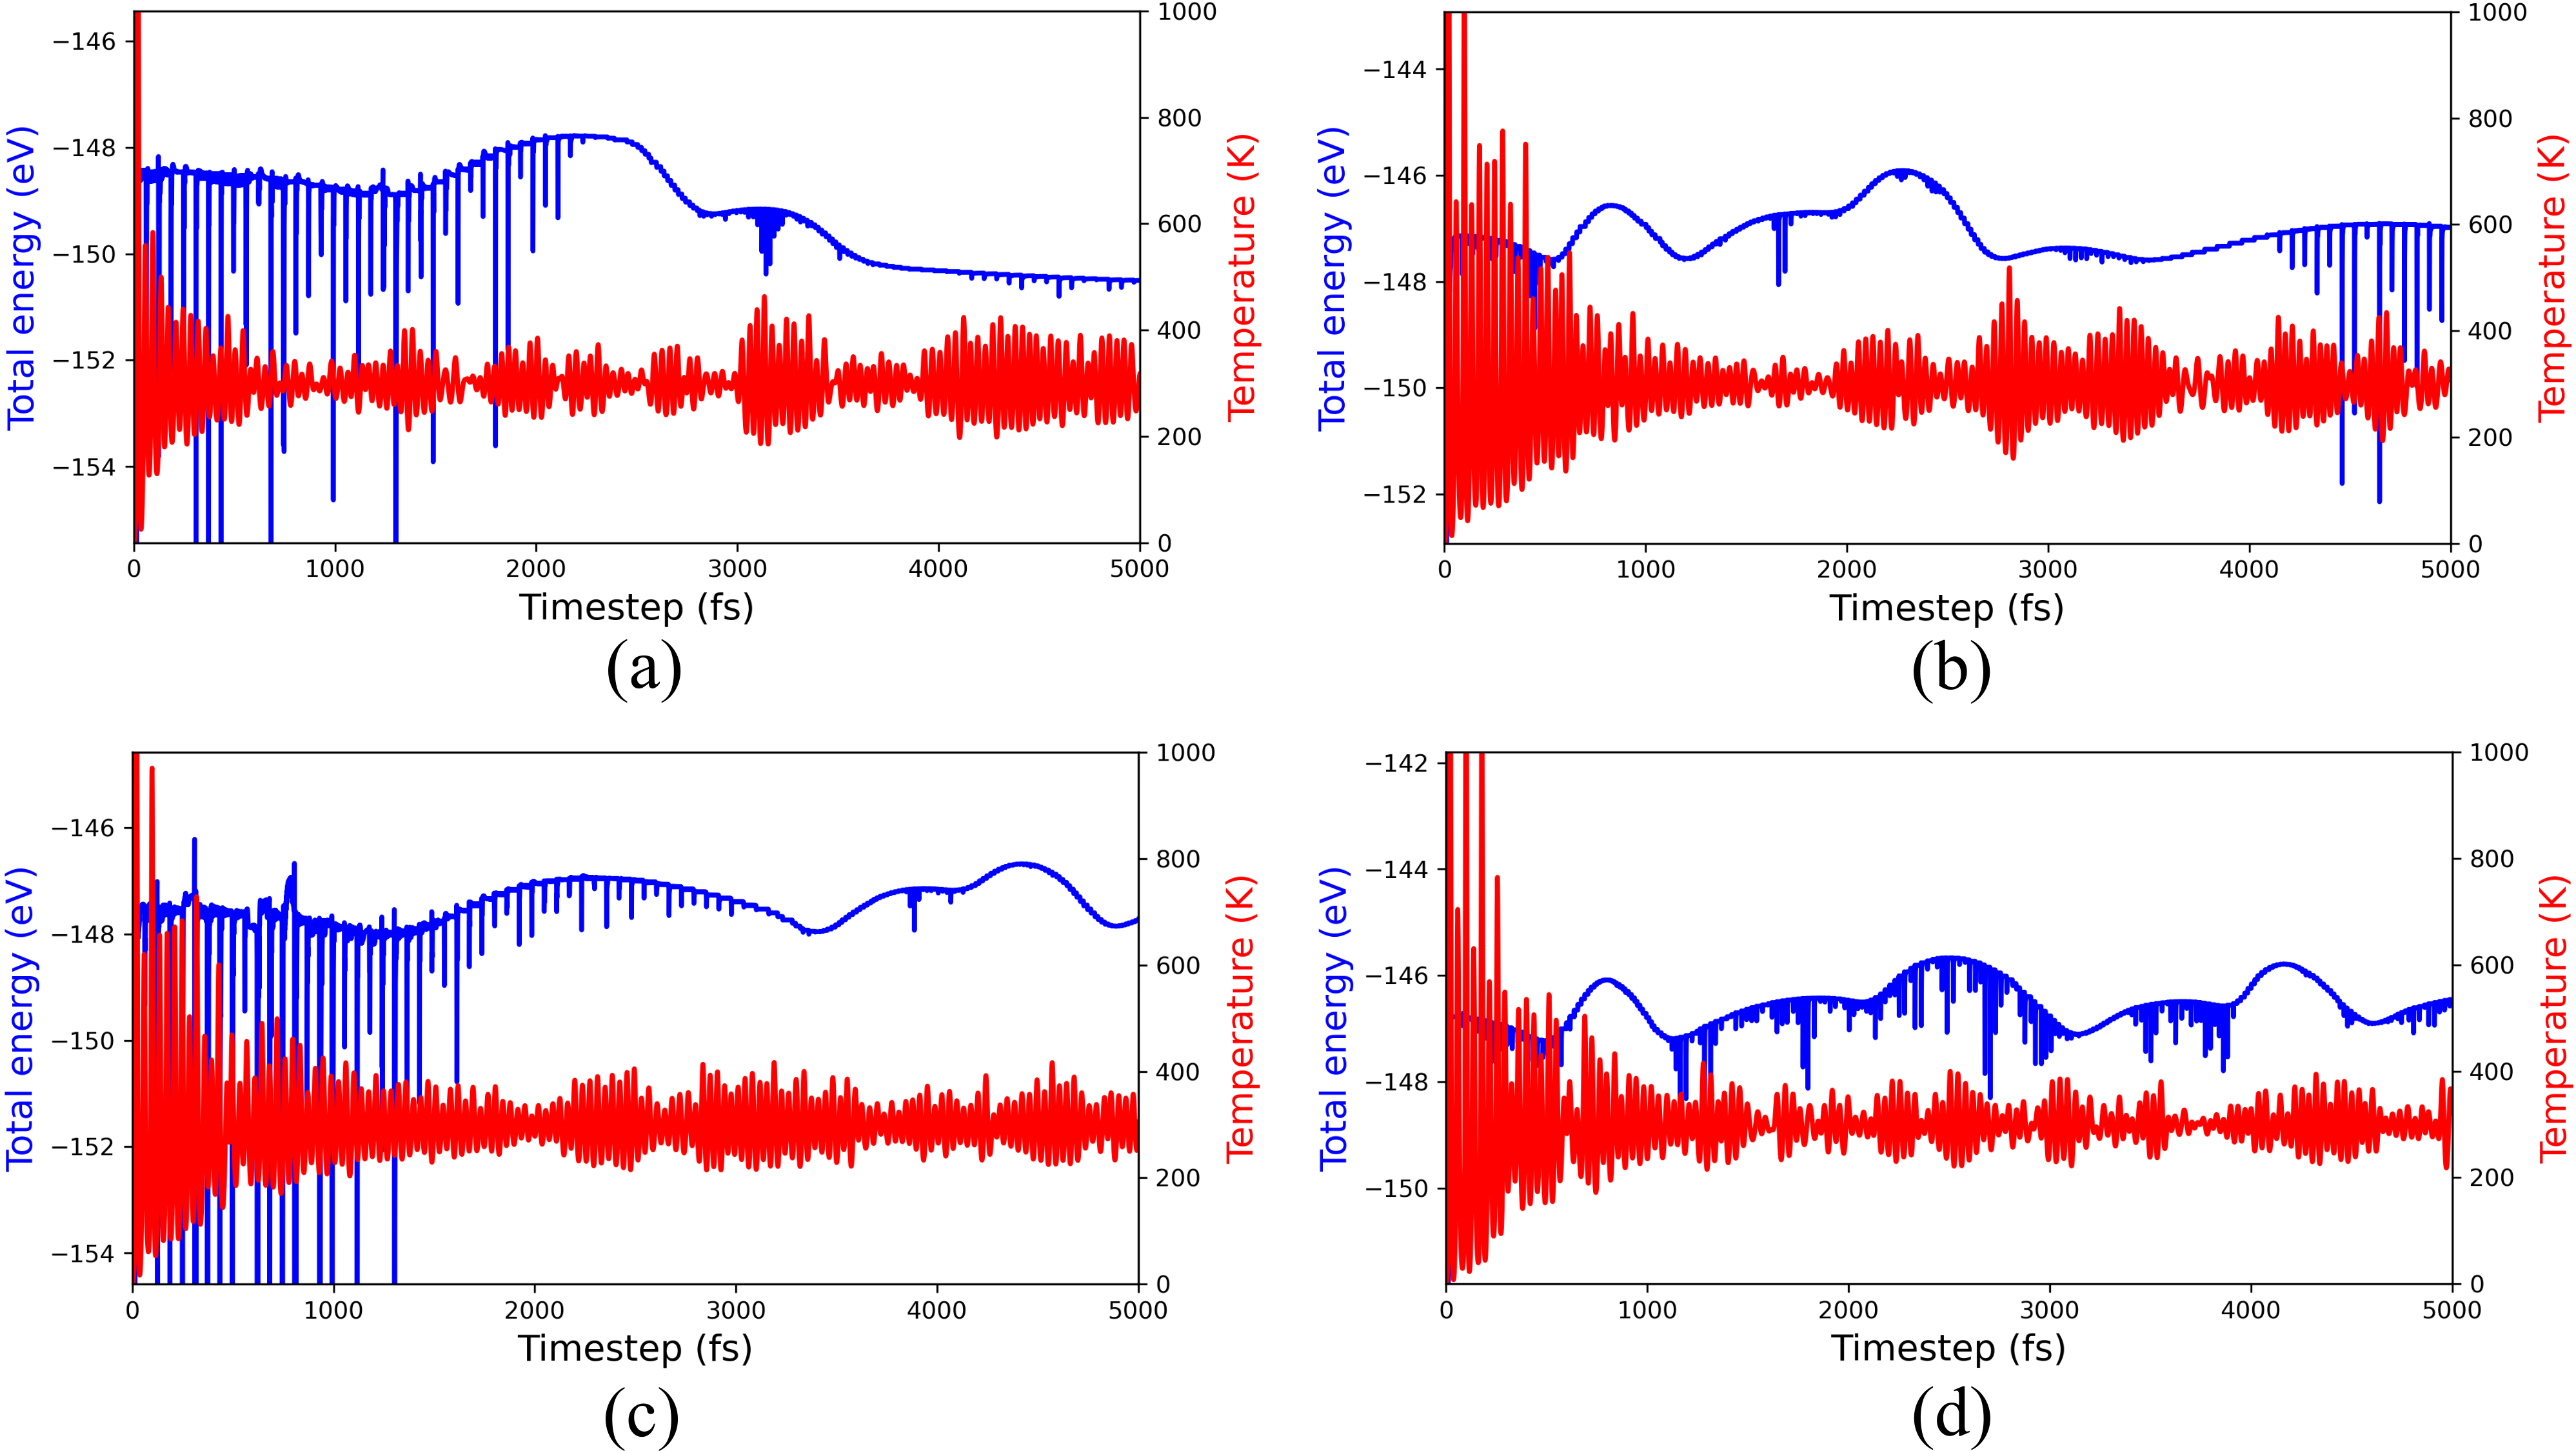
\includegraphics[width=1.0\linewidth]{figure/Fig_SI_3.png}
    \caption*{Fig. S3. Time evolution of the total energy (blue curves, left axes) and instantaneous temperature (red curves, right axes) during the 5~ps AIMD simulations at 300~K for monolayer CrCl$_3$ containing an initially surface-adsorbed (a) Cr, (b) Co, (c) Fe, or (d) Ni atom at the hollow site. Following the initial thermostatting  transients, the temperatures fluctuate around the target value. The changes in the total-energy profiles accompany the structural rearrangements sampled during the trajectories.}
    \label{fig:S3}
\end{figure}

\begin{figure}[H]
    \centering
    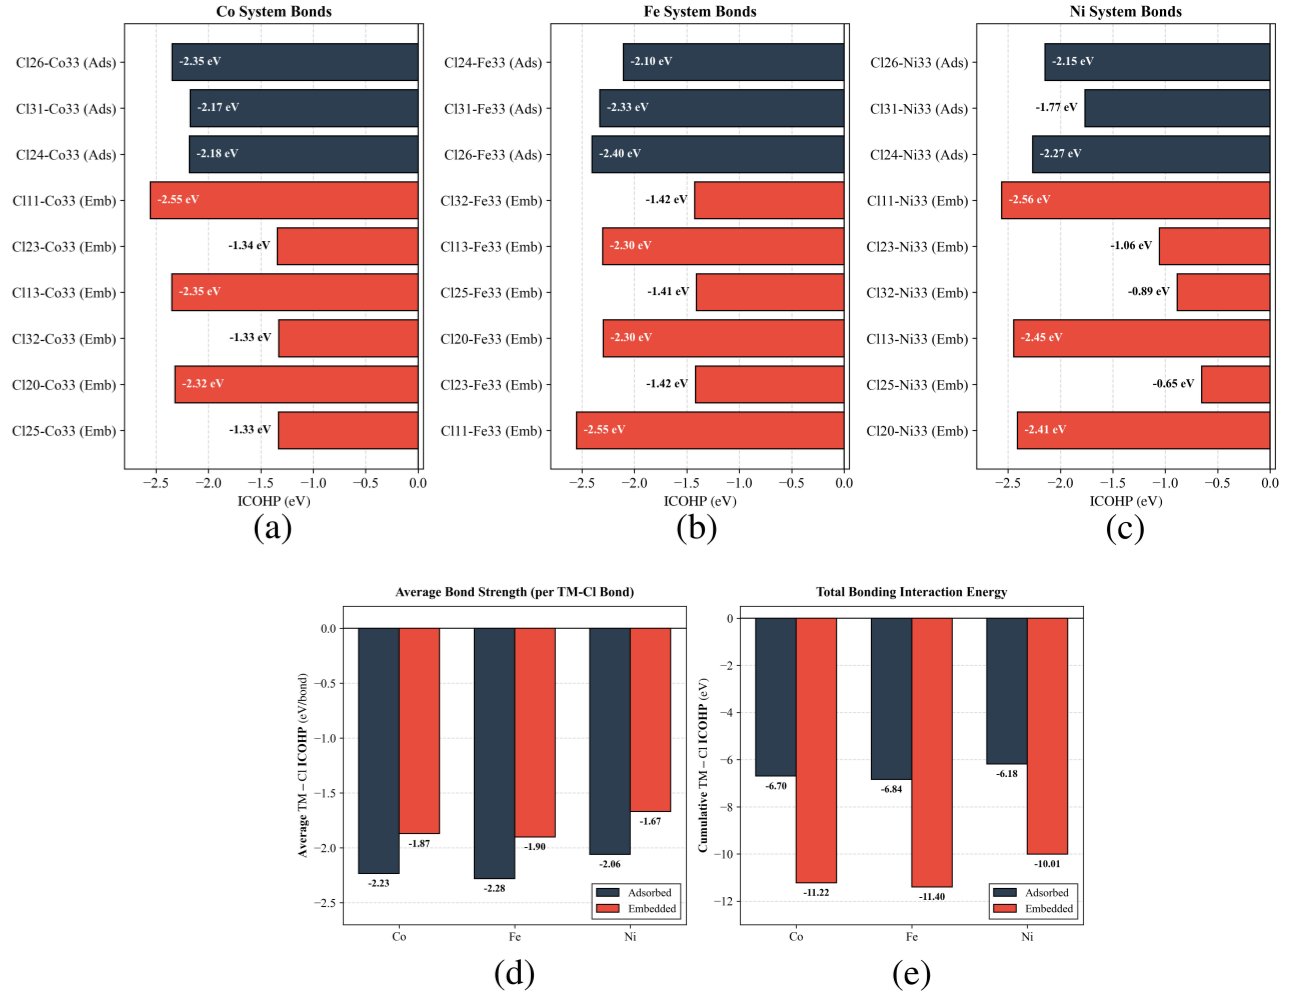
\includegraphics[width=0.95\textwidth]{figure/new_sup_fig_4.png}
    \caption*{Fig. S4. TM--Cl chemical-bonding analysis and relative stability of surface-adsorbed and embedded transition-metal configurations in monolayer CrCl$_3$. (a--c) Individual integrated crystal orbital Hamilton population (ICOHP) values for the Co--Cl, Fe--Cl, and Ni--Cl interactions, respectively. Dark bars correspond to the threefold coordinated surface-adsorbed configurations, whereas red bars correspond to the sixfold coordinated embedded configurations. More negative ICOHP values indicate stronger net bonding interactions. (d) Average ICOHP per TM--Cl bond for the adsorbed and embedded configurations. (e) Cumulative TM-Cl ICOHP obtained by summing the individual ICOHP contributions over the corresponding coordination shell.}
    \label{fig:Fig7}
\end{figure}

\begin{figure}[H]
        \centering
        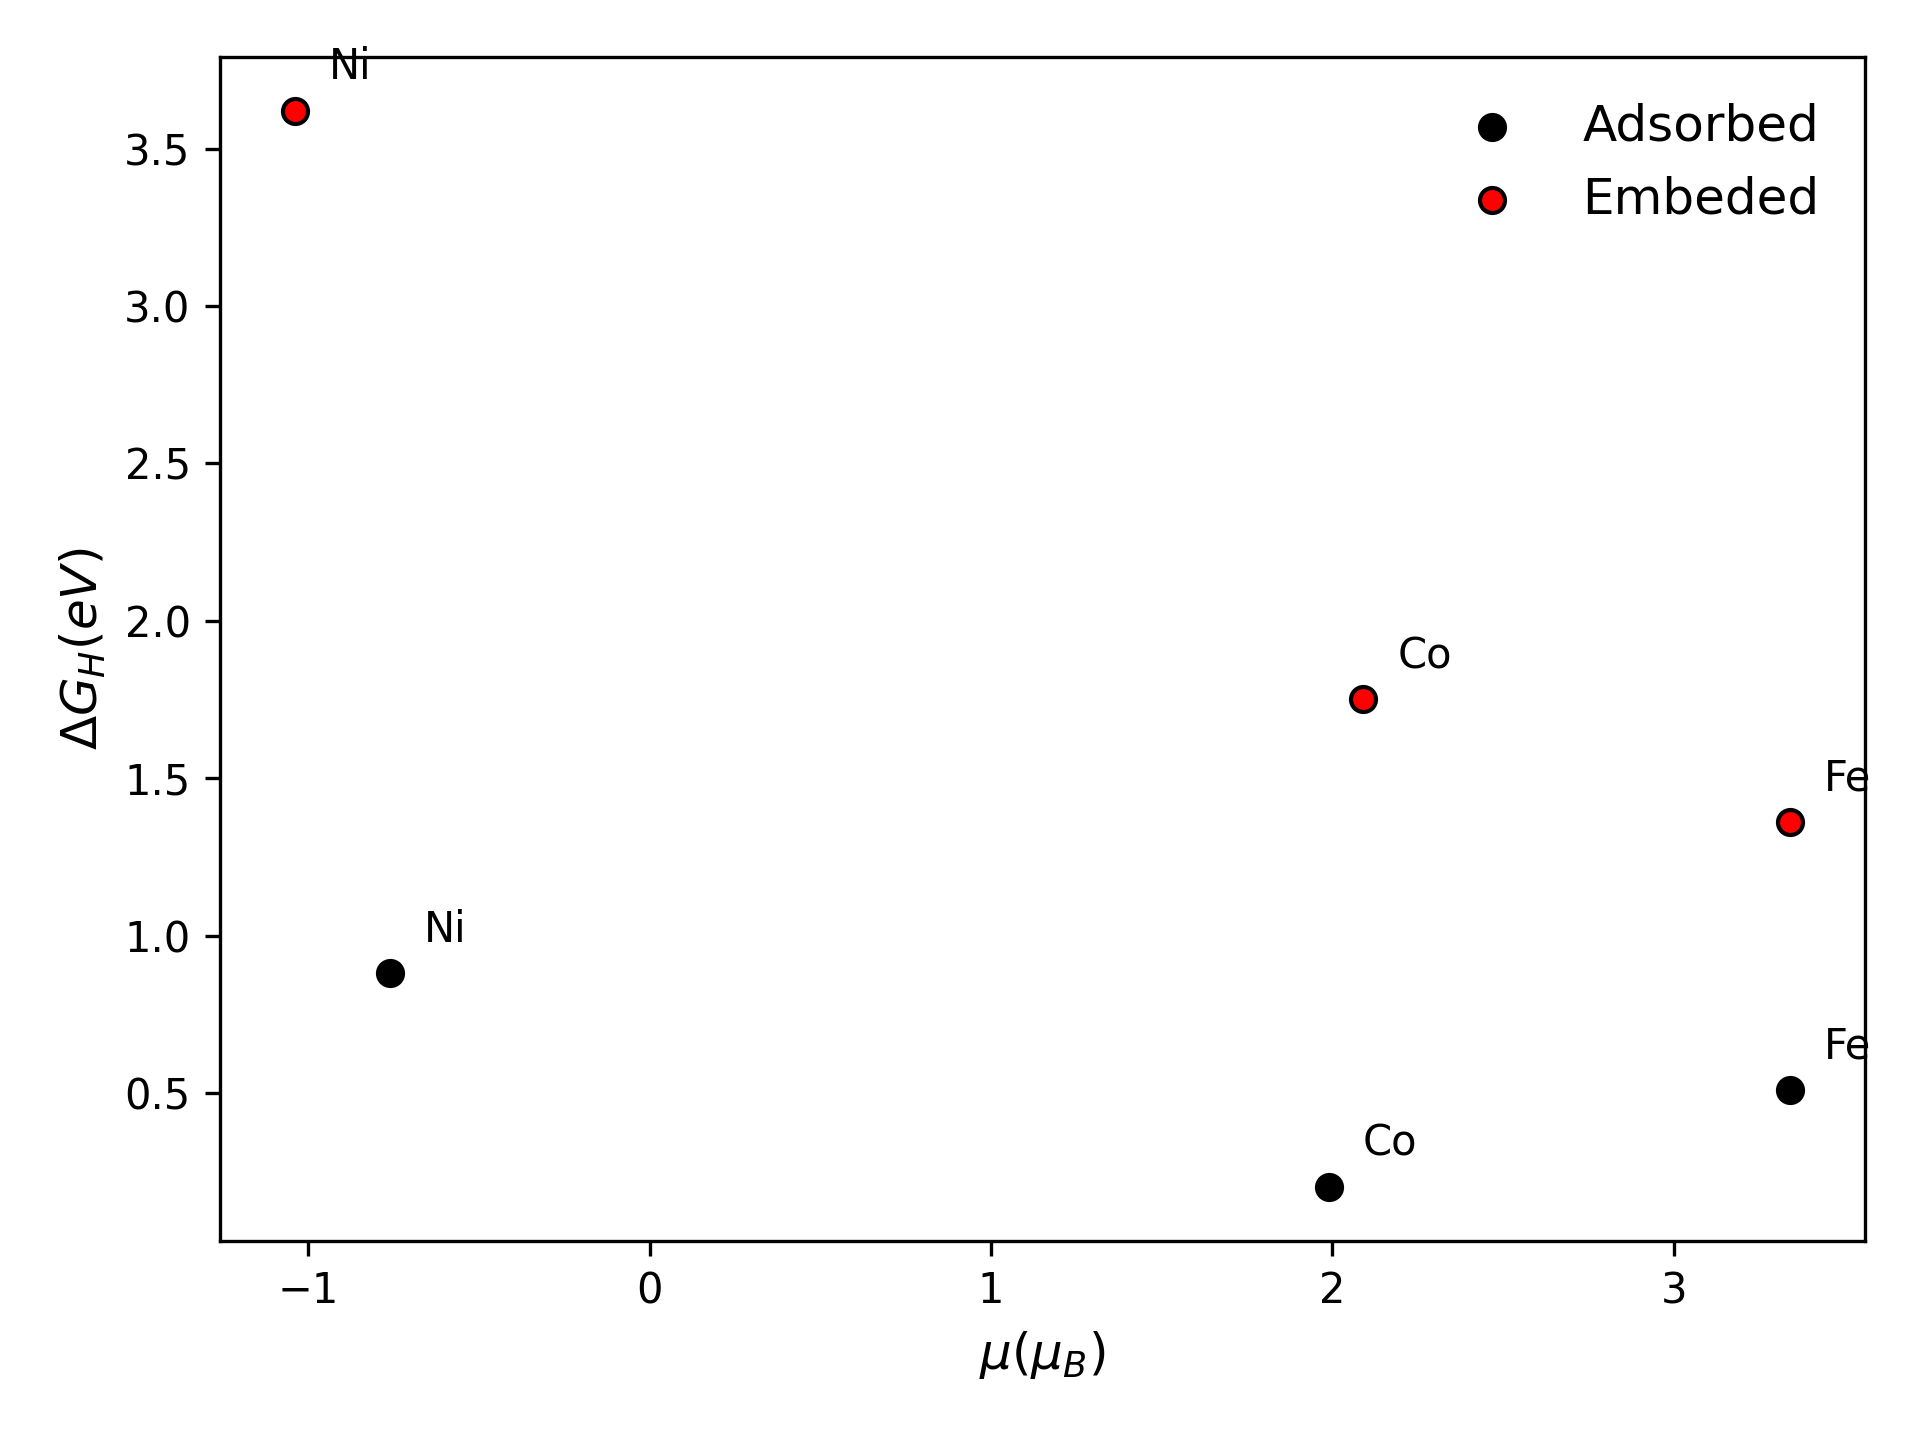
\includegraphics[width=0.8\linewidth]{figure/mu_vs_dG.png}
        \caption*{Fig. S5. Relationship between the local magnetic moment of the functionalizing transition-metal atom, $\mu_{\mathrm{TM}}$, in the relaxed H-free configurations and the hydrogen adsorption free energy, $\Delta G_{\mathrm{ads}}$, subsequently calculated after H adsorption. Black and red symbols represent the surface-adsorbed and embedded Co-, Fe-, and Ni functionalized CrCl$_3$ monolayers, respectively. Magnetic moments are expressed in units of the Bohr magneton, $\mu_{\mathrm{B}}$.}
        \label{fig:S5}
\end{figure}

\end{suppinfo}

\end{document}